\chapter{cta}
\label{cta}


\section{A short history of ground-based atmospheric cherenkov atronomy}
In the time between the discovery of cosmic radiation by Victor Hess (zitat)
and today there have been various different attempts to investigate its origins.
Experiments have been conducted in the form of Cherenkov teleskopes, scintilator 
arrays (beispiel mit zitat) and satelites. %unter anderem oder alles aufzählen?

To understand the motivation behind CTA, 
we will focus on the ground-based 
cherenkov telescopes and split our brief look at history 
into three generations as proposed by Turver and Weekes \cite{turver1980}.

During a Royal Society Meeting in 1981 they presented ways to improve on
the (at the time) current generation of telescopes by taking images of the shower
and exploiting stereoscopy with multiple telescopes.

\subsection{The first generation}
The first generation of cherenkov teleskopes 
lacked any kind of imaging as is present in all new experiments.
Instead they initially consisted of a single mirror with a single photomultiplier on top.
The first very simple attempt to catch the chernenkov light emitted by cosmic rays 
was done by Galbraith and Jelley in 1953 \cite{1953Natur.171..349G}, who found very few pulses
above background level.

A more sophisticated approach was later taken with the Whipple telescope \cite{whipple1968}:
It consisted of 252 small mirrors providing a large detector area and operated between 
1968 and 1976.
Later the telescope had multiple photomultipliers added to focus on the OFF- and ON-Region
at the same time and to reduce the sensitivity on hadronic showers by comparing
the light under different angles. (Hier brauchts irgendwie quellen...)

\subsection{The second generation}
To research the efectiveness of the "imaging-approach", in 1982 the groups around Fegan and Weekes
installed an imager consisting of 37 photomultipliers at the no longer used Whipple telescope.
This later got replaced by a more capable 109-pixel camera as can be seen in figure \ref{fig:whipple_cam}.

\begin{figure}
    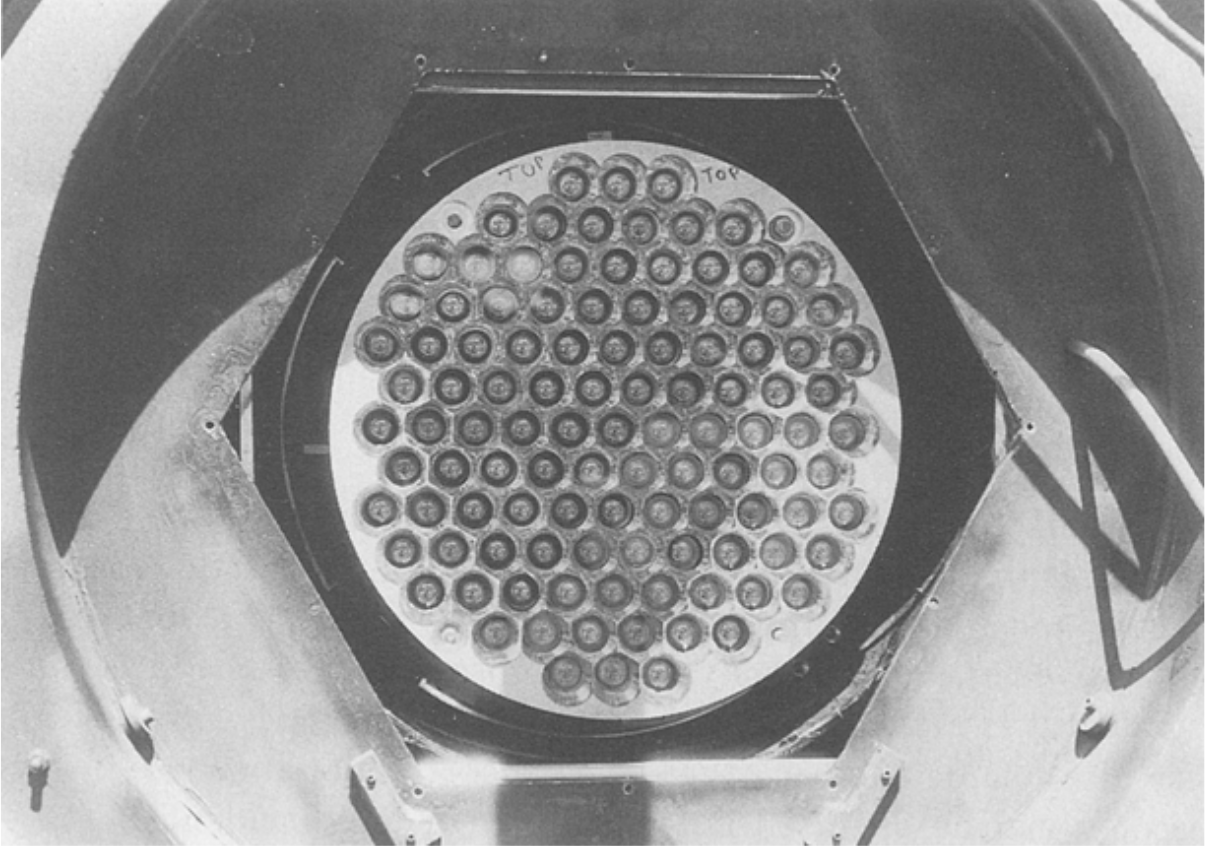
\includegraphics[width=0.8\textwidth]{images/whipple_cam.png}
    \caption{Picture of the upgraded camera of the Whipple telescope, installed in 1988 \cite{Cawley1995}.}  % not the best source
    \label{fig:whipple_cam}
\end{figure}

The shower images in combination with better computer simulations allowed for 
superior background rejection based on the  hillas-parameters [citation needed].

With this setup and the newly adopted analysis methods based on the pixel information , 
the Whipple group reported 45\sigma on the Crab Nebula with 68h of observatiopn time.

smth bout hegra


\subsection{The third generation}

Towards the end of the 1990s several third generation telescopes were
proposed:
H.E.S.S and MAGIC (-> zitate/verweise zu den experimenten), deriving from parts of the HEGRA collaboration, 
VERITAS from Whipple and the no longer operating CANGAROO from Adelaide and 
several japanese universities \cite{HILLAS201319}.
All of these were designed as stereoscopic imaging telescopes building on the progress made during the 
second generation with two experiments located on each north and south hemisphere.

\subsubsection{MAGIC}
MAGIC is a experiment initially operating as single telescope with a second slightly improved 
telescopes added later \cite{BAIXERAS2003247}.
Both telescopes have a 17m diameter, 964 elements mirror.

\subsubsection{H.E.S.S}

\subsubsection{VERITAS}

\subsubsection{CANGAROO}
gibts nicht mehr, also egal?



\section{Current Status/CTA}


% bis vlt seite 15-25
